\renewcommand{\baselinestretch}{1.25}%
\begin{figure}[!t]%
  \centering
  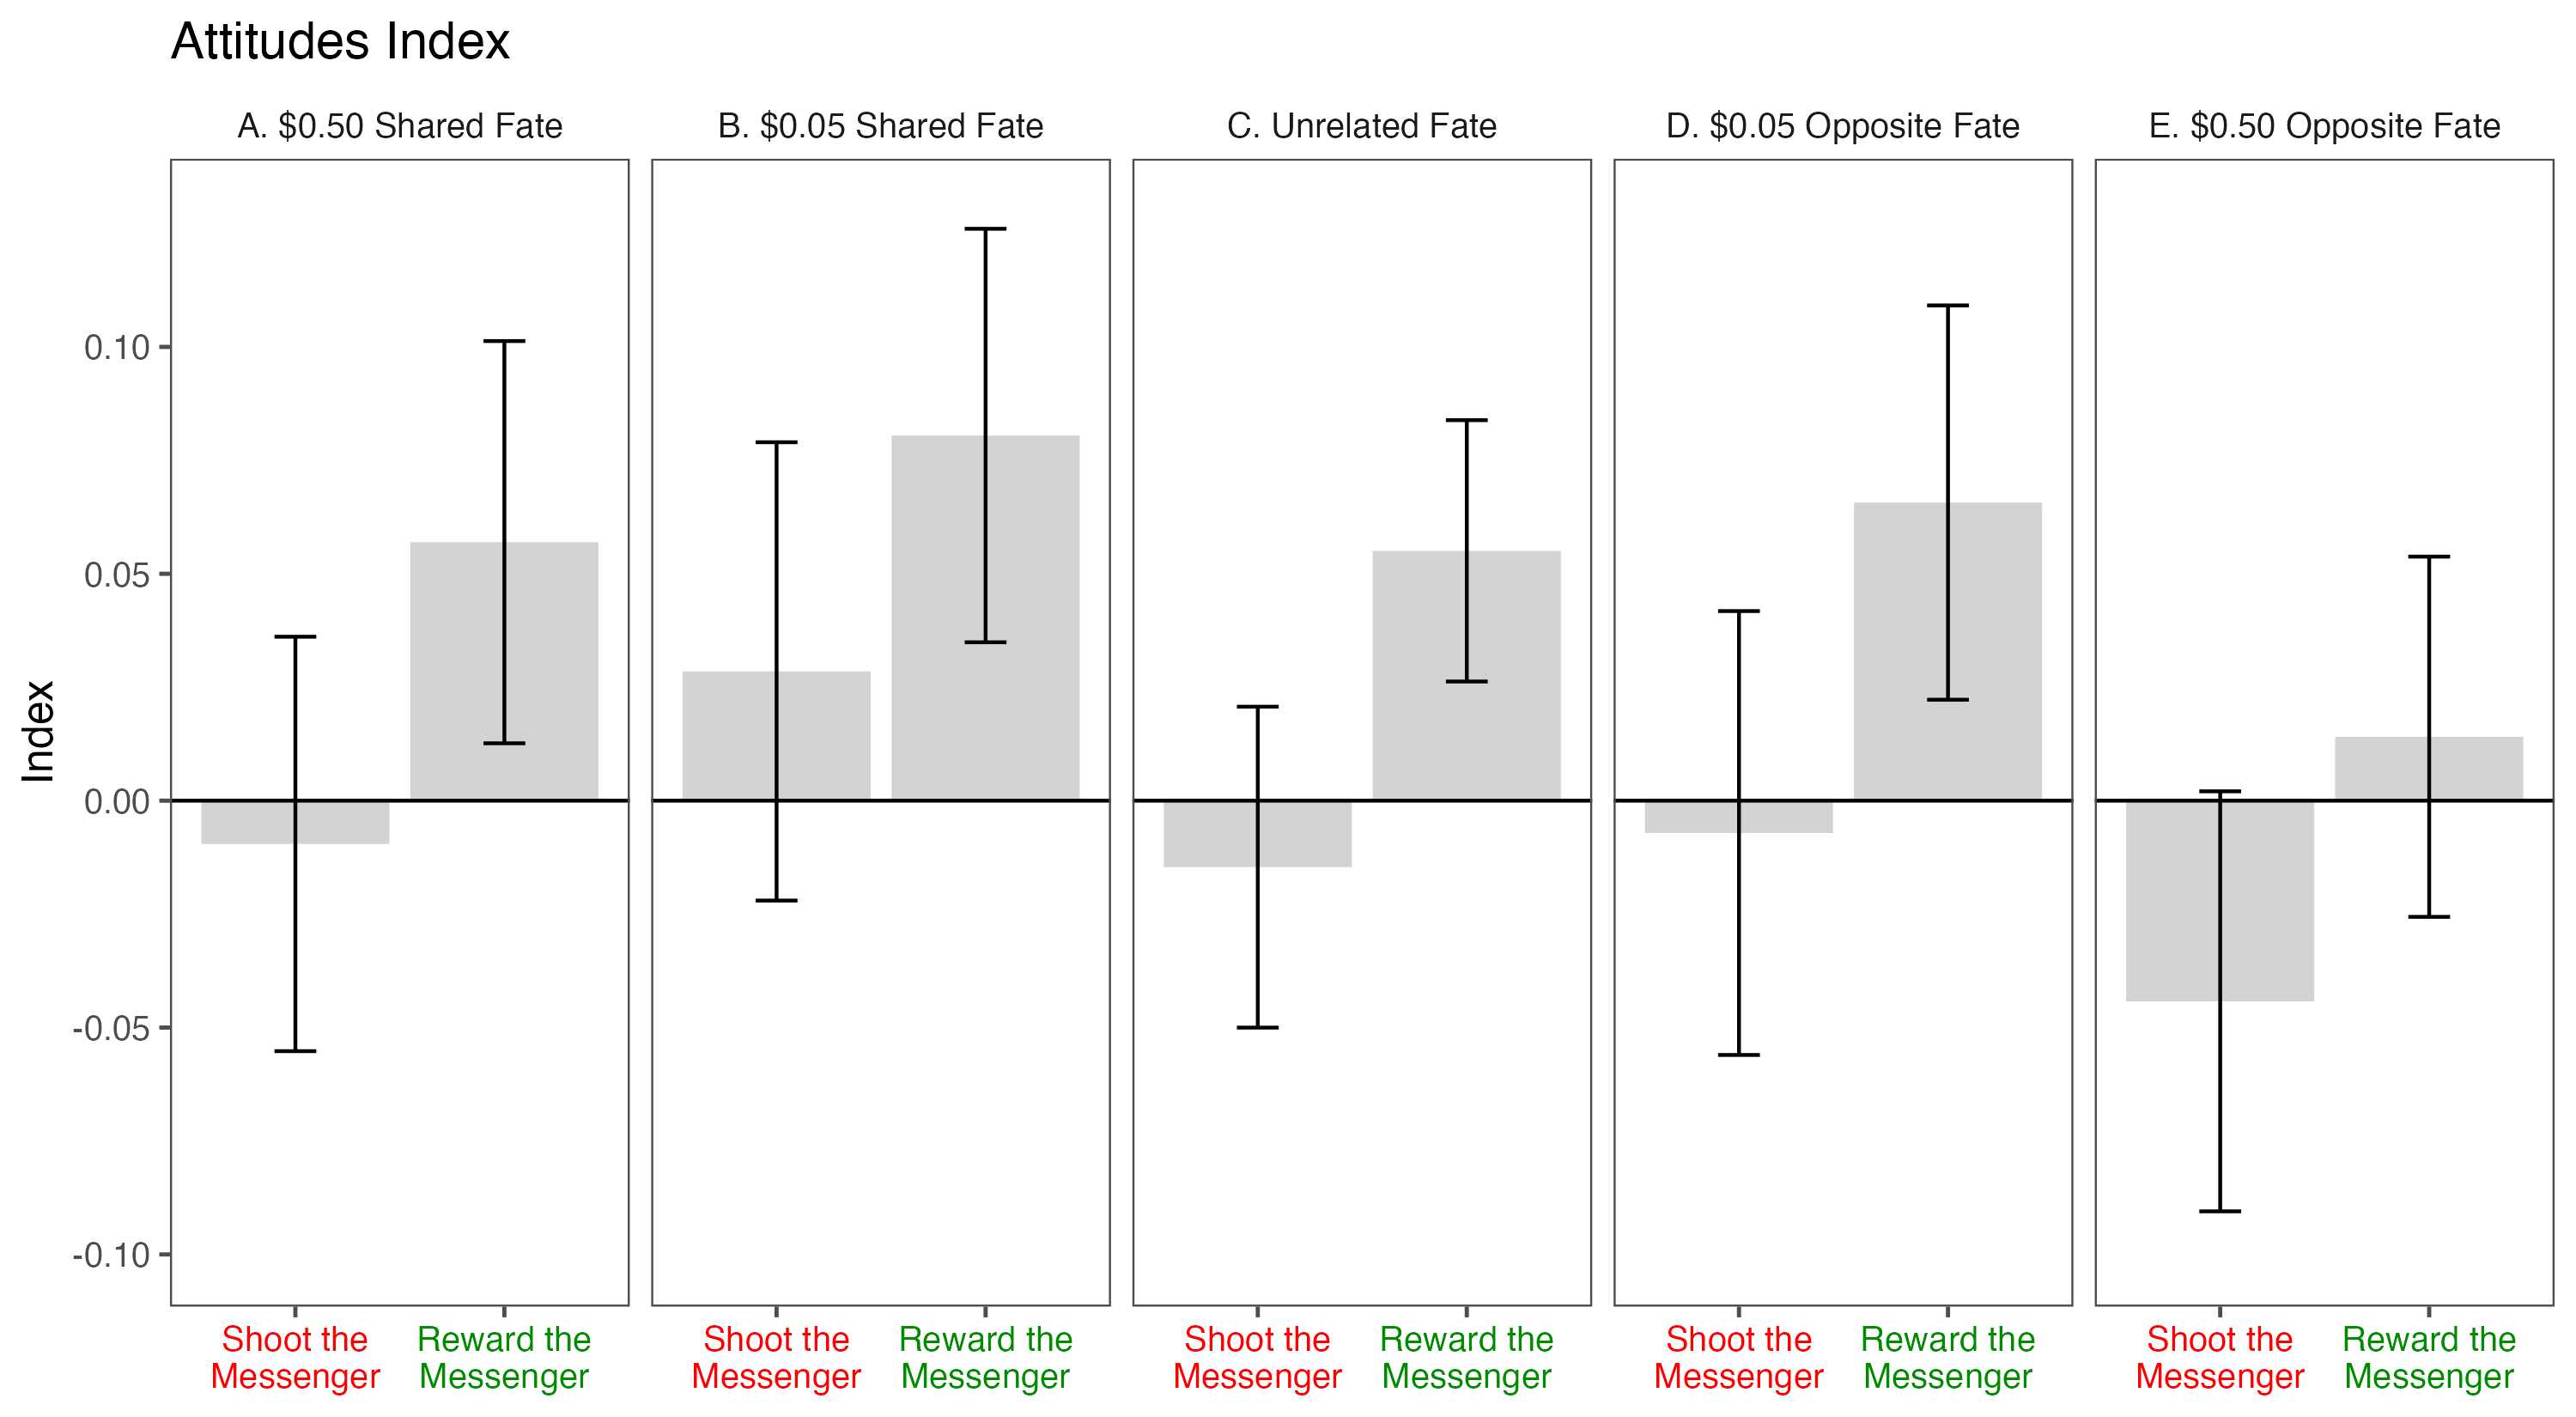
\includegraphics[width=1.0\textwidth]{figures/study2_main_fivecent_attitude_all.png}
  \caption{Difference in messenger and non-messenger ratings of the Attitudes Index by losing (STM) and winning (RTM) across unrelated fate, shared fate, opposite fate conditions, Study 2 (including 5 and 50 cent differences). 
  \textit{Note: OLS regression with robust standard errors, with error bars representing 95\% confidence intervals.In the attitudes index, the DV is calculated by averaging the ratings of the trustworthy, nice, likeable, and generous DVs to an index ranging from 0 to 1. The \$0.05 Shared Fate (Panel A) and \$0.50 Shared Fate (Panel B) conditions are when the partner wins \$0.05 or \$0.50, respectively, when the respondent wins. The Unrelated Fate (Panel C) condition is when the partner winnings are unrelated to the respondent winning. The \$0.05 Opposite Fate (Panel D) and \$0.50 Opposite Fate (Panel E) conditions are when the partner wins \$0.05 or \$0.50, respectively, when the respondent loses.}}
  \label{fig:study2_main_fivecent_attitude_all}
\end{figure}%
\renewcommand{\baselinestretch}{1.67}%
